\begin{enumerate}
% มุมระหว่างเวกเตอร์
\item \textbf{มุมระหว่างเวกเตอร์} 
ถ้ากำหนดมุมระหว่างเวกเตอร์ $\vec{v}, \vec{u}$ มีค่าเท่ากับ $\theta$ แล้วจะได้
\[ \cos \theta =  \rule{100pt}{.5pt}\]
หรือถ้าเราต้องการค่ามุม $\theta$ จะได้ $\theta = \rule{150pt}{.5pt}$

กำหนดให้มุมระหว่างเวกเตอร์แต่ละคู่มีค่าเท่ากับ $\theta$ แล้วจงหา $\cos\theta$
\begin{tasks}[after-item-skip = 80pt, after-skip = 80pt](2)
\task $\bv{1,3}$ และ $\bv{3,1}$
\task $\bv{-1, 2}$ และ $\bv{2, 1}$
%\task $\bv{3,-2}$ และ $\bv{-6, 4}$
%\task $\bv{4, 2}$ และ $\bv{2, 1}$
\end{tasks}

% การฉายเชิงตั้งฉาก (orthogonal projection)
\item \textbf{การฉายเชิงตั้งฉาก (orthogonal projection)} 

กำหนดเวกเตอร์ $\vec{u}$ และ $\vec{b}$ แล้วเราสามารถเขียน
\[ \vec{u} = \vec{w_1} + \vec{w_2}\]
โดยที่ 
\begin{itemize}
\item $\vec{w_1}$ คือ \rule{100pt}{.5pt} เขียนแทนด้วย \rule{100pt}{.5pt} มีสูตรเป็น \rule{100pt}{.5pt}
\item  $\vec{w_2}$ คือ \rule{100pt}{.5pt} มีสูตรเป็น \rule{100pt}{.5pt}
\end{itemize}

กำหนดเวกเตอร์ $\vec{u}$ และ $\vec{b}$ จงคำนวณส่วนประกอบของเวกเตอร์ $\vec{u}$ ตาม $\vec{b}$ และส่วนประกอบของเวกเตอร์ $\vec{u}$ ที่ตั้งฉากต่อ $\vec{b}$ พร้อมทั้งวาด $\vec{u}, \vec{b}, \vec{w_1}$ และ $\vec{w_2}$ ลงไปในกราฟที่กำหนดให้โดยคร่าว

\begin{tasks}(2)
\task $\vec{u} = \bv{3,2}, \vec{b} = \bv{2,0} $

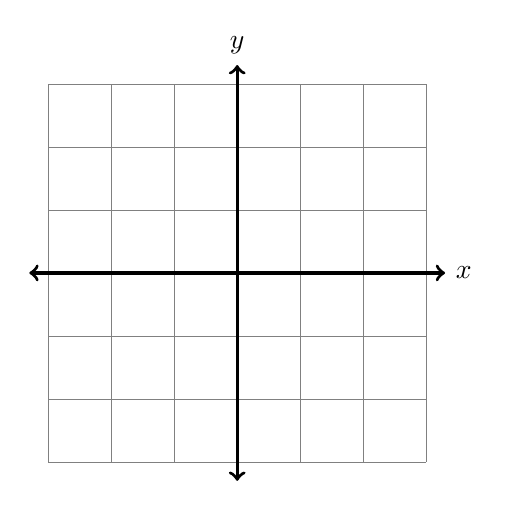
\begin{tikzpicture}[scale = 0.8]
\draw[help lines] (-3,-3) grid (3,3);
\draw[<->, very thick] (-3.3,0) -- (3.3,0) node[right] {$x$};
\draw[<->, very thick] (0,-3.3) -- (0,3.3) node[above] {$y$};
\end{tikzpicture}

\task $\vec{u} = \bv{-3,4}, \vec{b} = \bv{-4,3} $

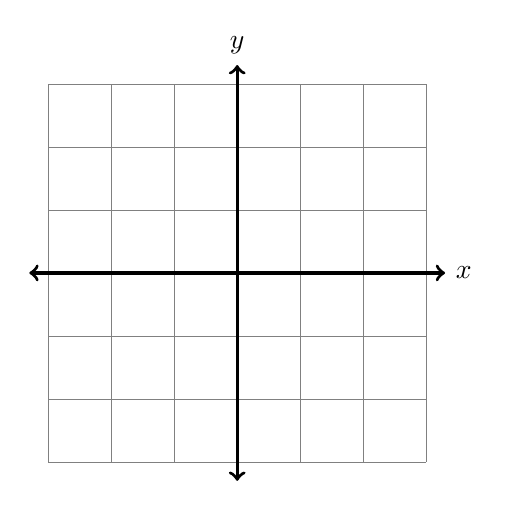
\begin{tikzpicture}[scale = 0.8]
\draw[help lines] (-3,-3) grid (3,3);
\draw[<->, very thick] (-3.3,0) -- (3.3,0) node[right] {$x$};
\draw[<->, very thick] (0,-3.3) -- (0,3.3) node[above] {$y$};
\end{tikzpicture}
\end{tasks}

\iffalse
\task $\vec{u} = \bv{0,1}, \vec{b} = \bv{-1,1} $

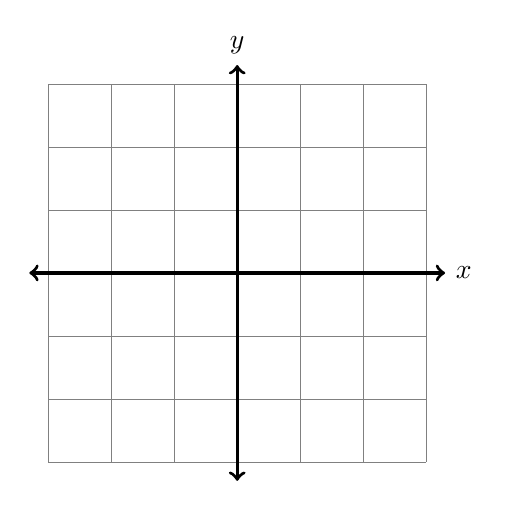
\begin{tikzpicture}[scale = 0.8]
\draw[help lines] (-3,-3) grid (3,3);
\draw[<->, very thick] (-3.3,0) -- (3.3,0) node[right] {$x$};
\draw[<->, very thick] (0,-3.3) -- (0,3.3) node[above] {$y$};
\end{tikzpicture}
\fi

\newpage
% ผลคูณไขว้
\item \textbf{ ผลคูณไขว้} 

กำหนดเวกเตอร์ $\vec{u} = \bv{u_1, u_2, u_3}$ และ $\vec{v} = \bv{v_1, v_2, v_3}$ แล้ว
\[\rule{20pt}{.5pt} \times \rule{20pt}{.5pt} = \begin{vmatrix} \hphantom{aaaaaaaa} \\  \\  \end{vmatrix} = \rule{100pt}{.5pt}\]

จงคำนวนผลคูณไขว้ของเวกเตอร์ที่กำหนดให้ต่อไปนี้
\begin{tasks}(2)
\task $\bv{1,0,2} \times \bv{0,3,4}$
\task $\bv{1,1,1} \times \bv{0,2,3}$
\end{tasks}
\vspace{100pt}

\mathnote{สมบัติที่สำคัญของผลคูณไขว้คือ $\vec{u} \times \vec{v}$ จะ \rule{50pt}{.5pt} กับ \rule{20pt}{.5pt} และ \rule{20pt}{.5pt} เสมอ}
% ผลคูณไขว้
\item \textbf{ประยุกต์ผลคูณไขว้}

กำหนดเวกเตอร์ $\vec{u}$ และ $\vec{v}$ ที่มีมุมระหว่างเวกเตอร์ทั้งสองเป็น $\theta$ แล้ว
\[ \sin \theta =  \rule{100pt}{.5pt} \]  

กำหนดเวกเตอร์ $\vec{u}$ และ $\vec{v}$ แล้วสี่เหลี่ยมด้านขนานที่เกิดจากเวกเตอร์ $\vec{u}$ และ $\vec{v}$ มีพื้นที่เท่ากับ
\[A = \rule{100pt}{.5pt}\]

กำหนดเวกเตอร์ $\vec{u}, \vec{v}$ และ $\vec{w}$ แล้วทรงสี่เหลี่ยมด้านขนานที่สร้างจากด้าน $\vec{u}, \vec{v}$ และ $\vec{w}$ จะปริมาตรค่าเท่ากับ
\[V = \rule{100pt}{.5pt}\]


จงหาค่า $\sin \theta$ ของเวกเตอร์ $\vec{u}$ และ $\vec{v}$ ที่กำหนดให้ต่อไปนี้
\begin{tasks}(2)
\task $\vec{u} = \bv{1,1,0}, \vec{v} = \bv{1,0,1} $
\vspace{50pt}
\task $\vec{u} = \bv{-3,0,4}, \vec{v} = \bv{4,0,3} $
\end{tasks}
\end{enumerate}
